\documentclass[a4paper,10pt]{article}
\usepackage[utf8]{inputenc}
\usepackage[margin=1.5cm, bottom=2cm]{geometry}
\usepackage{fancyhdr}
\usepackage[table]{xcolor}
\usepackage{enumitem}
\usepackage{xcolor}
\usepackage{makeidx}
\usepackage[most]{tcolorbox}
\newtcolorbox{osservazioni}{
  colback=gray!8,    % sfondo grigio chiaro
  colframe=white,      % nessun bordo
  arc=2mm,            % angoli smussati
  boxrule=0pt,        % spessore bordo 0
  fontupper=\footnotesize,
  left=2mm, right=2mm, top=2mm, bottom=2mm,
  before skip=7pt,   % niente spazio prima
  after skip=15pt     % niente spazio dopo
}
\newtcolorbox{osservazioni2}{
  colback=gray!8,    % sfondo grigio chiaro
  colframe=white,      % nessun bordo
  arc=2mm,            % angoli smussati
  boxrule=0pt,        % spessore bordo 0
  fontupper=\small,
  left=5mm, right=5mm, top=3mm, bottom=3mm,
  before skip=0pt,   % niente spazio prima
  after skip=30pt     % niente spazio dopo
}
\pagestyle{fancy}
\usepackage{tikz}
\usetikzlibrary{automata, positioning}
\pagestyle{fancy}

\usepackage{makeidx}

%%%%%%%%%%%%%%%%%%%
\newcommand{\EsercitazioneNum}{09}
\newcommand{\Data}{04/11/2025}
\newcommand{\DocType}{Esercitazione} % o "Eserciziario"
\newcommand{\FullTitle}{\DocType\ \EsercitazioneNum}

\newcommand{\Header}{
\noindent
  \small \textbf{Computabilità, Complessità e Logica - a.a. 2025/26} \hfill \textbf{\FullTitle} \\[0.2cm]
  \scriptsize Matteo Liotta, \texttt{matteo.liotta@studenti.units.it} \hfill \Data \\[0.2cm]
  \noindent\makebox[\linewidth]{\rule{\linewidth}{0.4pt}} \\[0.3cm]}

\newcommand{\NewPageHeader}{
  \vfill
  \noindent\makebox[\linewidth]{\rule{\linewidth}{0.4pt}}
  \newpage
  {\Header}
}
%%%%%%%%%%%%%%%%%%%

% Numero di pagina in basso al centro
\fancyhf{}
\fancyfoot[C] \thepage
\renewcommand{\footrulewidth}{0pt} % niente linea in basso
\renewcommand{\headrulewidth}{0pt} % niente linea in alto

\begin{document}

\footnotesize  % font generale più piccolo
\Header\\[0.7cm]


%%%%%%%%%%%%%%%% FOGLIO 2


%% INDEX
\addcontentsline{toc}{section}{Esercitazione 07: \textit{Macchine di Turing}}

\noindent\Large \textbf{Esercitazione 9}: \textit{Macchine di Turing (cont'd)}
\begin{osservazioni}
    \textbf{\textit{Nota}}. Sono indicati in \textcolor{blue}{\textit{blu}} gli esercizi che non saranno trattati durante l'esercitazione, bensì lasciati come strumento aggiuntivo di esercitazione individuale. Resta comunque assoluta disponibilità per la loro risoluzione negli incontri successivi, qualora necessario.
\end{osservazioni}

{\normalsize
\begin{itemize}[label=, leftmargin=0pt]

    %% INDEX
    \addcontentsline{toc}{subsection}{Esercizio 52.} 
    %%
    \item \textbf{Esercizio 52 (*)}\\ Sia $L$ linguaggio su $\Sigma=\{a,b\}$ (cfr. \textit{approfondimento 02}), tale per cui:
    {\begin{center}
        $L=\{w\#w'| w,w'\in\Sigma^*, \quad \exists i \in \mathbf{N} \quad t.c.\quad  w(i)=w'(i)\ \}$
    \end{center}} 
    Si rappresenti la macchina di Turing tale da riconoscere il linguaggio $L$.\\[0.1cm]

    
    %% INDEX
    \addcontentsline{toc}{subsection}{Esercizio 53.} 
    %%
    \item \textbf{\textcolor{black}{Esercizio 53.} (*)}\\ Sia $L$ linguaggio su $\Sigma=\{a,b,c\}$, tale per cui 
    {\begin{center}
        $L = \{ x\#y \mid x,y\in\Sigma^*\quad e \quad x \text{ prefisso di }y\}$
    \end{center}}
    Si rappresenti la macchina di Turing tale da riconoscere il linguaggio $L$.\\[0.1cm]

    
    %% INDEX
    \addcontentsline{toc}{subsection}{Esercizio 54.} 
    %%
    \item \textbf{\textcolor{blue}{Esercizio 54.} (*)}\\ Sia $L$ linguaggio su $\Sigma=\{a,b,c\}$, tale per cui 
    {\begin{center}
        $L = \{ x\#y \mid x,y\in\Sigma^*\quad e \quad x \text{ sottostringa di }y\}$
    \end{center}}
    Si rappresenti la macchina di Turing tale da riconoscere il linguaggio $L$.\\[0.1cm]
    
    %% INDEX
    \addcontentsline{toc}{subsection}{Esercizio 55.} 
    %%
    \item \textbf{\textcolor{orange}{Esercizio 55.} (***)}\\ 
    Si considerino le seguenti identificazioni, considerando il seguente alfabeto $\{0,1\}$ e simboli ausiliari $\{\$_1,\$_2,\$_c,\#_1,\#_2,\sqcup\}$:
    \begin{itemize}[label=\textbullet]
        \item \texttt{00} $\equiv$ \texttt{IF} $\quad \mid \quad $ \texttt{01} $\equiv$ \texttt{ELSE}
        \item \texttt{0} $\equiv$ \texttt{$\leq$} $\quad \mid \quad $ \texttt{1} $\equiv$ \texttt{$>$}
        \item \texttt{10} $\equiv$ \texttt{AND} $\quad \mid \quad $ \texttt{1} $\equiv$ \texttt{OR (element-wise)}
    \end{itemize}
    Dove sono presenti le seguenti regole sintattiche:
    \begin{itemize}[label=\textbullet]
        \item Ogni operazione di controllo con if richiede l'indicazione del termine di paragone voluto, i termini da confrontare, correttamente separati:\\ \texttt{IF [binary num 1]  [binary num 2] CONFRONTO THEN [what to do]} $\equiv$ 
        \texttt{IF$\$_1x\$_2y\$_cc\#_1command\#_2$} \\{$x,y\in\Sigma^*$}
        \item Si definisce l'operazione alternativa, posta dopo la codifica del THEN dell'IF:\\ \texttt{ELSE [what to do]} $\equiv$ \texttt{ELSE$\#_1command\#_2$}
        \item Mentre, con operazioni (then), in questo caso si sono considerate somme e sottrazioni elementwise degi termini:\\ \texttt{OPERATION [binary num 1] [binary num 2]} $\equiv$ 
        \texttt{OP$\$_1x\$_2y\#_2 \quad x,y\in\Sigma^*$}
        
    \end{itemize}
    Si scriva una macchina di Turing che, ricevendo in input una stringa del programma (vedi esempio), ritorni sul nastro il risultato finale dell'(ultima) operazione

\item \textit{e.g.} \textit{Se 010 $>$ 001 allora effettuane l'AND}: \begin{itemize} \item \texttt{INPUT: 00$\$_1$010$\$_2$001$\$_c$1$\#_1$10$\$_1$010$\$_2$001$\#_2$} \item \texttt{OUTPUT: 011} \end{itemize}

\NewPageHeader
\begin{osservazioni}
\underline{\textit{Soluzione.}}\\
Consideriamo dapprima che, all'inizio, possiamo sempre solo osservare quattro casistiche: \texttt{00,01,10,11}:

    {
    \small
    \begin{center}
	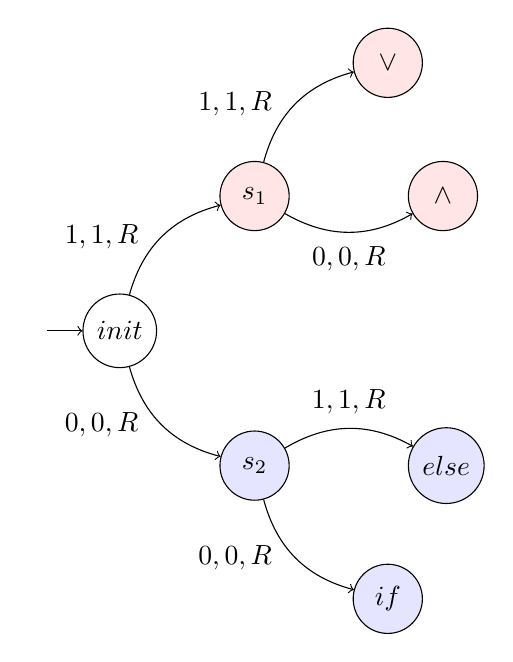
\begin{tikzpicture}
		
        \node[state, initial, initial text=] (s0) {$init$};
		\node[state] (s1) [above right=1.5of s0, fill=red!10] {$s_1$};
		\node[state] (s2) [below right=1.5of s0, fill=blue!10] {$s_2$};

        \node[state] (s3) [right=1.5of s2, fill=blue!10] {$else$};
		\node[state] (s4) [below right=1.5of s2, fill=blue!10] {$if$};

        \node[state] (s5) [right=1.5of s1, fill=red!10] {$\land$};
		\node[state] (s6) [above right=1.5of s1, fill=red!10] {$\lor$};

		\path[->] 
        (s0) edge[left, bend left] node {$\begin{array}{c} 1,1,R\end{array}$} (s1)
        (s0) edge[left, bend right] node {$\begin{array}{c} 0,0,R\end{array}$} (s2)

        (s2) edge[above, bend left] node {$\begin{array}{c} 1,1,R\end{array}$} (s3)
        (s2) edge[left, bend right] node {$\begin{array}{c} 0,0,R\end{array}$} (s4)

        (s1) edge[below, bend right] node {$\begin{array}{c} 0,0,R\end{array}$} (s5)
        (s1) edge[left, bend left] node {$\begin{array}{c} 1,1,R\end{array}$} (s6);

    \end{tikzpicture}
    \end{center}
    }
A questo punto, ricordiamo che nel caso di IF ci aspettiamo anche un confronto, che sarà indicato da $1/0$. Sarebbe utile costruire una sottoporzione specializzata della macchina, tale da mappare in due nodi in cui viene mantenuta l'informazione implicita del rapporto tra i numeri. In questo modo, tramite la semplice lettura del termine di confronto successivo, potremo mappare in uno stato in cui è mantenuta la situazione di verità del confronto. \\

Per farlo, consideriamo dapprima il controllo binario element-wise: poiché stiamo considerando numeri binari, è sufficiente che la macchina controlli il \textit{primo elemento per cui i numeri differiscono}; il primo dei due che avrà $1$, sarà il maggiore. \\

Consideriamo la lettura del primo numero, in cui ricordiamo:
\begin{itemize}
    \item Se $w_1(1:i-1) =w_2(1:i-1)$ e $w_1(i)=1,w_2(i) =0$ allora $w_1>w_2$
    \item Se $w_1(1:i-1) =w_2(1:i-1)$ e $w_1(i)=0,w_2(i) =1$ allora $w_1<w_2$
    \item Se $w_1(1:i-1) =w_2(1:i-1)$ e $w_1(i)=0,w_2(i) =0 $ o $1\quad \forall i$ allora $w_1=w_2$
\end{itemize}

{
    \small
    \begin{center}
	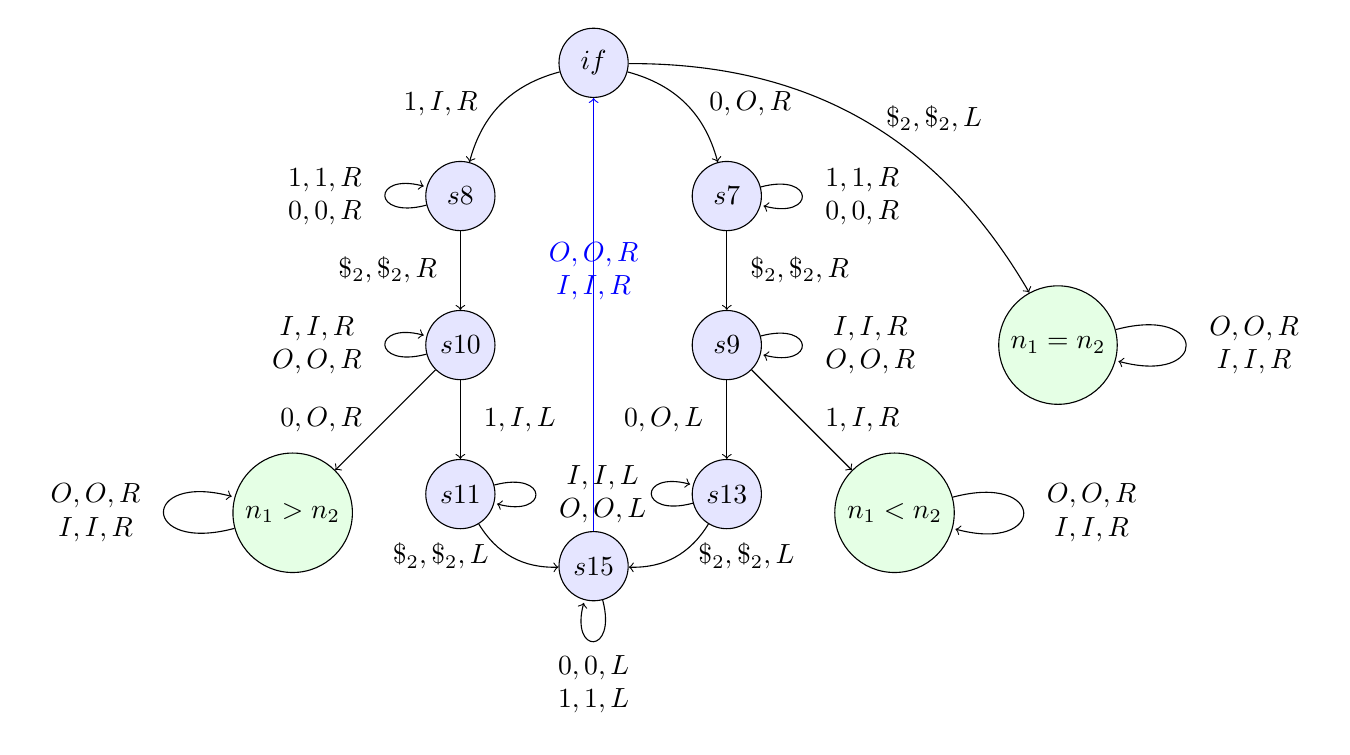
\begin{tikzpicture}
		
		\node[state] (s4) [fill=blue!10] {$if$};
        \node[state] (s7) [below right=1.5 of s4, fill=blue!10] {$s7$};
        \node[state] (s8) [below left=1.5 of s4, fill=blue!10] {$s8$};
        \node[state] (s9) [below=1 of s7, fill=blue!10] {$s9$};
        \node[state] (s10) [below=1 of s8, fill=blue!10] {$s10$};
        \node[state] (s12) [below left=1.8 of s10, fill=green!10] {$n_1>n_2$};
        \node[state] (s11) [below=1 of s10, fill=blue!10] {$s11$};
        \node[state] (s13) [below =1 of s9, fill=blue!10] {$s13$};
        \node[state] (s14) [below right =1.8 of s9, fill=green!10] {$n_1<n_2$};
        \node[state] (s16) [right =3 of s9, fill=green!10] {$n_1=n_2$};
        \node[state] (s15) [below =5.5 of s4, fill=blue!10] {$s15$};

		\path[->] 
        (s4) edge[right, bend left] node {$\begin{array}{c} 0,O,R\end{array}$} (s7)
        (s4) edge[left, bend right] node {$\begin{array}{c} 1,I,R\end{array}$} (s8)
        (s8) edge[left, loop left] node {$\begin{array}{c} 1,1,R \\ 0,0,R\end{array}$} (s8)
        (s7) edge[left, loop right] node {$\begin{array}{c} 1,1,R \\ 0,0,R\end{array}$} (s7)
        (s8) edge[left] node {$\begin{array}{c} \$_2,\$_2,R\end{array}$} (s10)
        (s7) edge[right] node {$\begin{array}{c} \$_2,\$_2,R\end{array}$} (s9)
        (s10) edge[left, loop left] node {$\begin{array}{c} I,I,R \\ O,O,R\end{array}$} (s8)
        (s9) edge[left, loop right] node {$\begin{array}{c} I,I,R \\ O,O,R\end{array}$} (s7)

        (s9) edge[right] node {$\begin{array}{c} 1,I,R\end{array}$} (s14)
        (s9) edge[left] node {$\begin{array}{c} 0,O,L\end{array}$} (s13)

        (s10) edge[right] node {$\begin{array}{c} 1,I,L\end{array}$} (s11)
        (s10) edge[left] node {$\begin{array}{c} 0,O,R\end{array}$} (s12)

        (s11) edge[left, loop right] node {$\begin{array}{c} I,I,L \\ O,O,L\end{array}$} (s11)
        (s13) edge[left, loop left] node {} (s13)
        (s11) edge[left, bend right] node {$\begin{array}{c} \$_2,\$_2,L\end{array}$} (s15)
        (s13) edge[right, bend left] node {$\begin{array}{c} \$_2,\$_2,L\end{array}$} (s15)
        (s15) edge[below, loop below] node {$\begin{array}{c} 0,0,L\\1,1,L\end{array}$} (s15)
        (s15) edge[draw=blue, above] node[blue] {$\begin{array}{c} O,O,R\\I,I,R\end{array}$} (s4)

        (s4)  edge[right, bend left] node {$\begin{array}{c} \$_2,\$_2,L\end{array}$} (s16)

        (s14) edge[loop right] node {$\begin{array}{c} O,O,R\\I,I,R\end{array}$} (s14)
        (s12) edge[loop left ] node {$\begin{array}{c} O,O,R\\I,I,R\end{array}$} (s12)
        (s16) edge[loop right] node {$\begin{array}{c} O,O,R\\I,I,R\end{array}$} (s16);


    \end{tikzpicture}
    \end{center}
    }

\end{osservazioni}
\NewPageHeader
\begin{osservazioni}
A questo punto sappiamo in che situazione si trovano, rispetto al confronto, i due addendi, quando gestiti dall'IF. Questo controllo viene effettuato sui termini, ma solo a seguito della lettura del termine di confronto, $>\ o\ \leq$, potremo raggiungere uno stato in cui ci si riconduce alla condizione di verità propria della condizione dell'IF:

{
    \small
    \begin{center}
	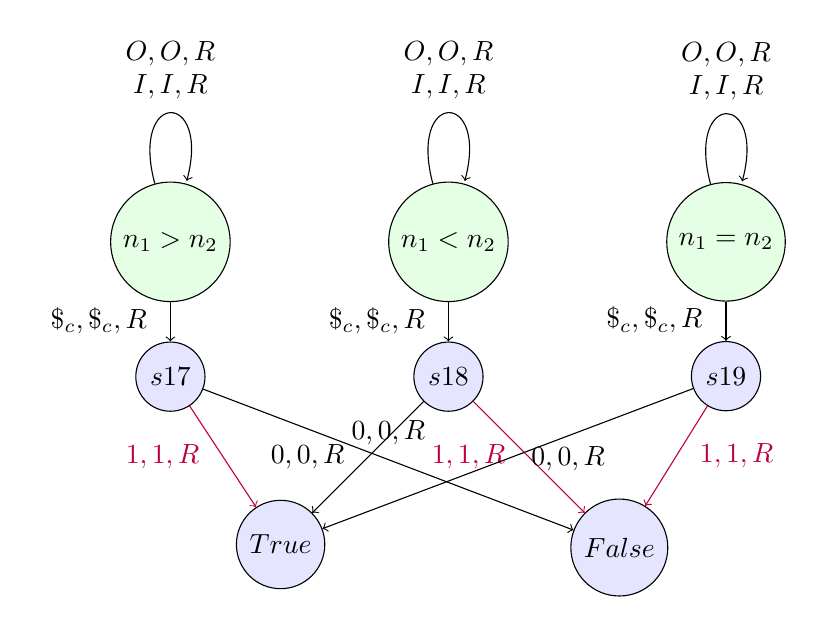
\begin{tikzpicture}
		
        \node[state] (s12) [fill=green!10] {$n_1>n_2$};
        \node[state] (s14) [right =2 of s12, fill=green!10] {$n_1<n_2$};
        \node[state] (s16) [right =2 of s14, fill=green!10] {$n_1=n_2$};

        \node[state] (s17) [below=0.5 of s12, fill=blue!10] {$s17$};
        \node[state] (s18) [below=0.5 of s14, fill=blue!10] {$s18$};
        \node[state] (s19) [below=0.5 of s16, fill=blue!10] {$s19$};
        \node[state] (s20) [below left =2 of s18, fill=blue!10] {$True$};
        \node[state] (s21) [below right =2 of s18, fill=blue!10] {$False$};
        


		\path[->] 

        (s14) edge[loop above] node {$\begin{array}{c} O,O,R\\I,I,R\end{array}$} (s14)
        (s12) edge[loop above] node {$\begin{array}{c} O,O,R\\I,I,R\end{array}$} (s12)
        (s16) edge[loop above] node {$\begin{array}{c} O,O,R\\I,I,R\end{array}$} (s16)

        (s12) edge[left] node {$\begin{array}{c} \$_c,\$_c,R \end{array}$} (s17)
        (s14) edge[left] node {$\begin{array}{c} \$_c,\$_c,R \end{array}$} (s18)
        (s16) edge[left] node {$\begin{array}{c} \$_c,\$_c,R \end{array}$} (s19)

        (s17) edge[left, draw=purple] node[purple] {$\begin{array}{c} 1,1,R \end{array}$} (s20)
        (s18) edge[left, draw=purple] node[purple] {$\begin{array}{c} 1,1,R \end{array}$} (s21)
        (s19) edge[right, draw=purple] node[purple] {$\begin{array}{c} 1,1,R \end{array}$} (s21)
        
        (s17) edge[above] node {$\begin{array}{c} 0,0,R \end{array}$} (s21)
        (s18) edge[left] node {$\begin{array}{c} 0,0,R \end{array}$} (s20)
        (s19) edge[right] node {$\begin{array}{c} 0,0,R \end{array}$} (s20);

    \end{tikzpicture}
    \end{center}
    }
Così, se ad esempio da $n_1>n_2$ osservo che il controllo era $>$ (codificato con 1), allora la condizione dell'IF è verificata. A questo punto, abbiamo una MDT che, ricevendo una codifica della forma \texttt{00$\$_1$010$\$_2$001$\$_c$1} sul nastro, riesce a ritornare, riesce a ritornare la condizione di verità (ossia a mappare ad uno stato in cui è contenuta implicitamente quella condizione, true o false). 


A questo punto mancano ancora la gestione della condizione THEN, la gestione dell'ELSE e la gestione delle operazioni element-wise. (Faremo riferimento al codice della precedente esercitazione per la costruzione di AND logico).

Si noti che:
\begin{itemize}
    \item Ci aspettiamo l'esecuzione di un \texttt{ELSE} solamente dopo la falsità della condizione
    \item Se a True, la sezione \textit{ELSE} dovrà essere ignorata. Ci aspettiamo che sia dopo il corpo dell'IF, come indicato in consegna. Si noti che, dopo aver eseguito una qualsiasi zona di operazioni, non ci aspettiamo di poter leggere 01 (else): sarà obbligatorio provenire da una condizione di verità. Dunque, se accade, salteremo tutti i termini fino a $\#_2$
    \item Quindi, se a False, \textit{ignoreremo tutto il corpo dell'}\texttt{IF}
\end{itemize}

Arriviamo, poiché ora più semplice, alla situazione in cui siamo pronti, in ambo i casi \texttt{IF/ELSE} a gestire per iniziare a considerare il relativo \texttt{THEN}. 


{
    \small
    \begin{center}
	\begin{tikzpicture}
		
        \node[state] (s20) [below left =1 of s18, fill=blue!10] {$True$};
        \node[state] (s21) [below right =1 of s18, fill=blue!10] {$False$};
        \node[state] (s22) [below=1 of s20, fill=black!10] {$s22$};
        \node[state] (s23) [below=1 of s21, fill=black!10] {$s23$};
        \node[state] (s24) [below=1 of s23, fill=black!10] {$s24$};
        
        \node[state] (s2) [below right=0.5of s0, fill=blue!10] {$s_2$};



		\path[->] 
        (s20) edge[left] node {$\begin{array}{c} \#_1,\#_1,R \end{array}$} (s22)
        (s21) edge[left] node {$\begin{array}{c} \#_1,\#_1,R \end{array}$} (s23)
        (s23) edge[loop right] node {$\begin{array}{c} 0,0,R\\1,1,R\\ \$_1,\$_1,R\\\$_2,\$_2,R \end{array}$} (s23)
        (s23) edge[left] node {$\begin{array}{c} \#_2,\#_2,R \end{array}$} (s24)
        (s24) edge[bend right, draw=red] node[red] {$\begin{array}{c} 0,0,R \end{array}$} (s2);
        
    \end{tikzpicture}
    \end{center}
    }

Si noti come la connesione rimanda, per semplicità al caso di biforcazione if/else. Ci aspettiamo comunque sia seguito da uno zero, ma si preferisce per evitare l'aggiunta di un nodo.
Questa che segue è la condizione corrente della costruzione: possiamo dire ora che siamo pronti a gestire e introdurre le operazioni element-wise.

\end{osservazioni}
\NewPageHeader
\begin{osservazioni}

{
    \small
    \begin{center}
	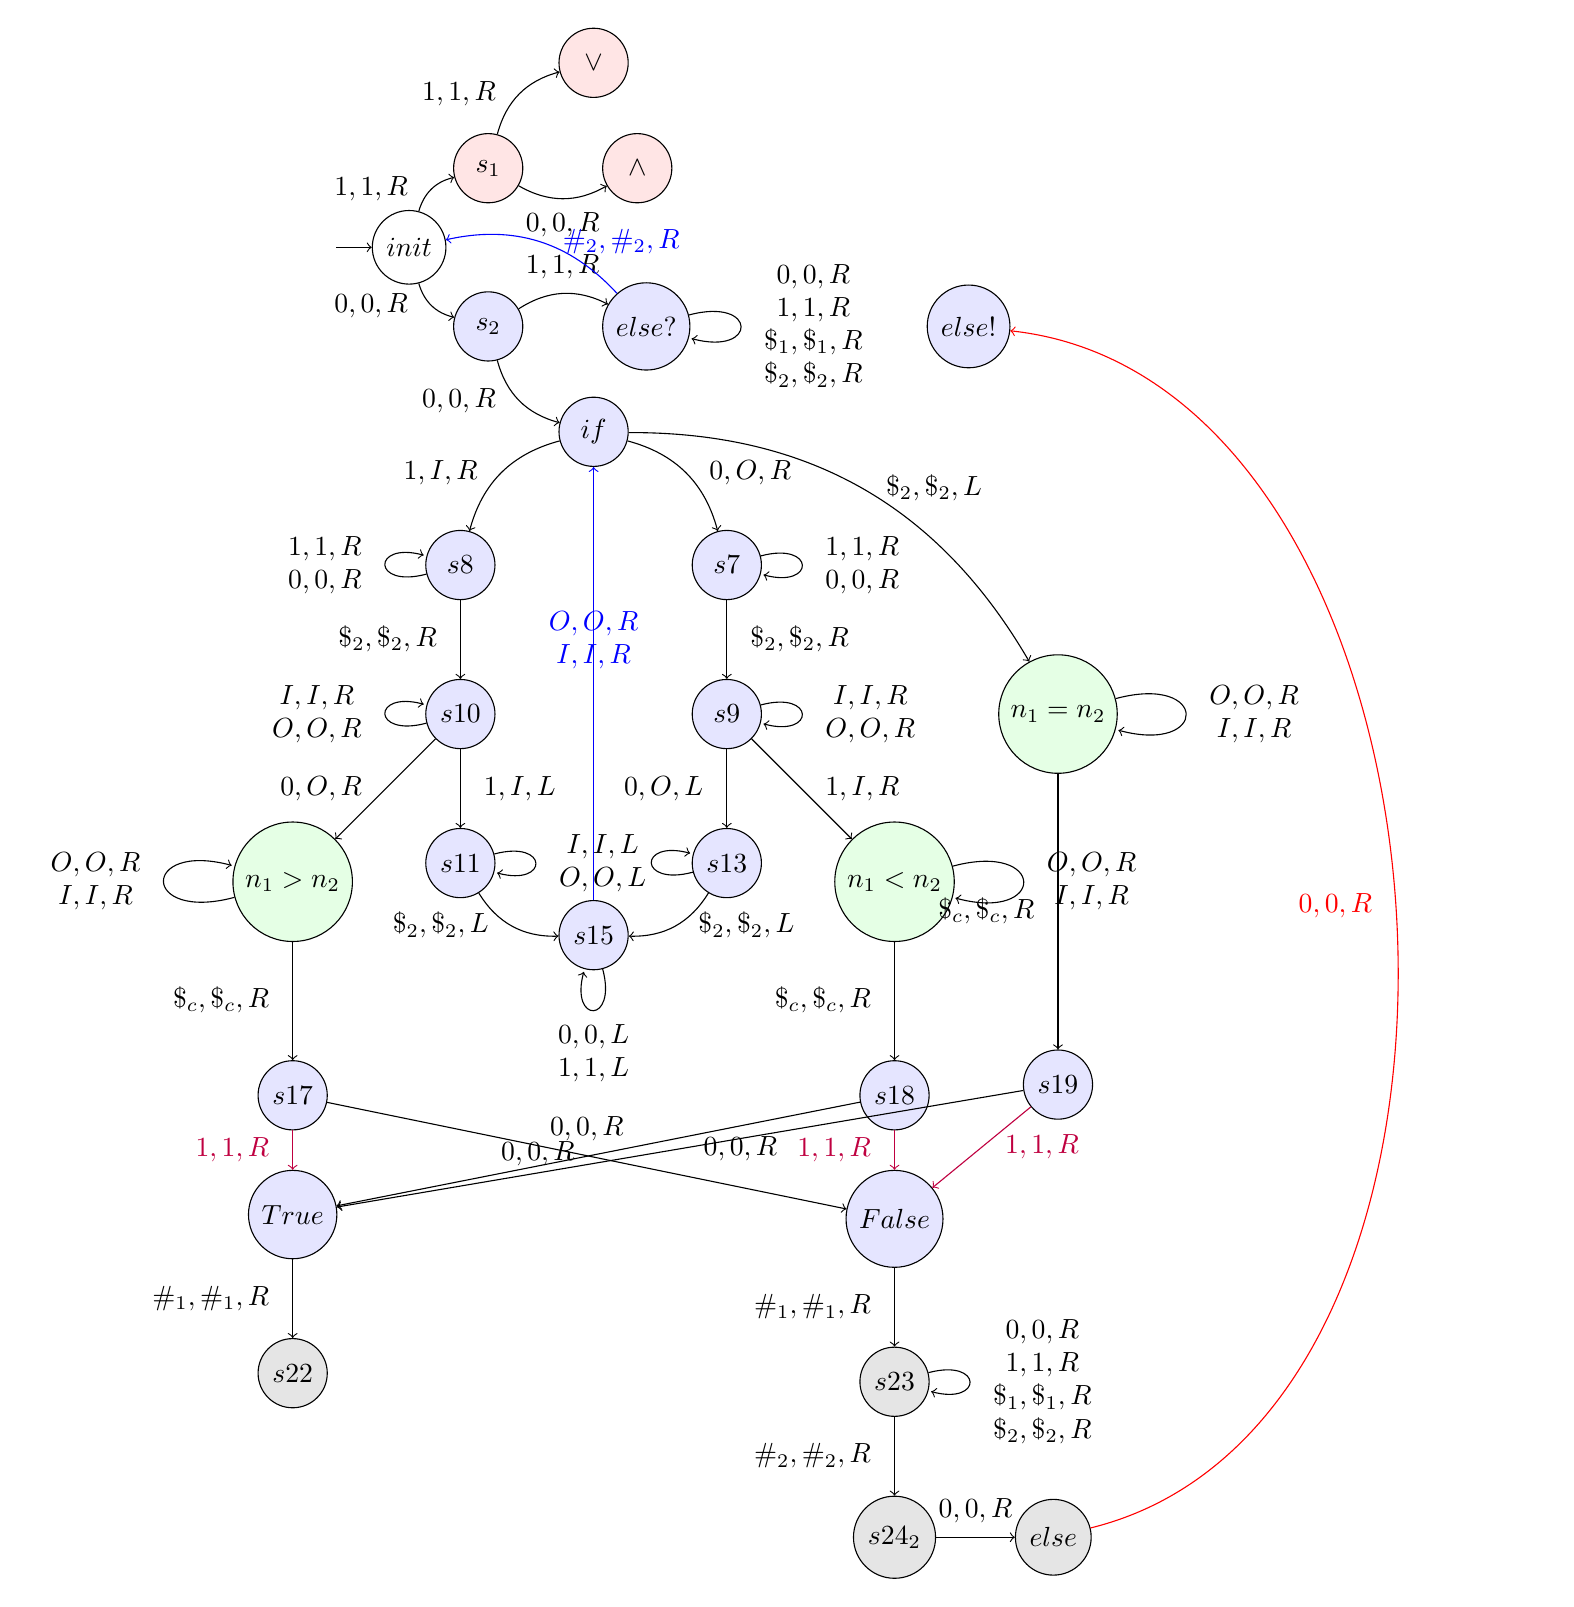
\begin{tikzpicture}
		
        \node[state, initial, initial text=] (s0) {$init$};
		\node[state] (s1) [above right=0.5of s0, fill=red!10] {$s_1$};
		\node[state] (s2) [below right=0.5of s0, fill=blue!10] {$s_2$};

        \node[state] (s3) [right=1of s2, fill=blue!10] {$else?$};
        \node[state] (s3_2) [right=3of s3, fill=blue!10] {$else!$};
		\node[state] (s4) [below right=1of s2, fill=blue!10] {$if$};

        \node[state] (s5) [right=1of s1, fill=red!10] {$\land$};
		\node[state] (s6) [above right=1of s1, fill=red!10] {$\lor$};

        \node[state] (s7) [below right=1.5 of s4, fill=blue!10] {$s7$};
        \node[state] (s8) [below left=1.5 of s4, fill=blue!10] {$s8$};
        \node[state] (s9) [below=1 of s7, fill=blue!10] {$s9$};
        \node[state] (s10) [below=1 of s8, fill=blue!10] {$s10$};
        \node[state] (s12) [below left=1.8 of s10, fill=green!10] {$n_1>n_2$};
        \node[state] (s11) [below=1 of s10, fill=blue!10] {$s11$};
        \node[state] (s13) [below =1 of s9, fill=blue!10] {$s13$};
        \node[state] (s14) [below right =1.8 of s9, fill=green!10] {$n_1<n_2$};
        \node[state] (s16) [right =3 of s9, fill=green!10] {$n_1=n_2$};
        \node[state] (s15) [below =5.5 of s4, fill=blue!10] {$s15$};

        \node[state] (s17) [below=1.5 of s12, fill=blue!10] {$s17$};
        \node[state] (s18) [below=1.5 of s14, fill=blue!10] {$s18$};
        \node[state] (s19) [below=3.5 of s16, fill=blue!10] {$s19$};
        \node[state] (s20) [below =0.5 of s17, fill=blue!10] {$True$};
        \node[state] (s21) [below =0.5 of s18, fill=blue!10] {$False$};

        \node[state] (s22) [below=1 of s20, fill=black!10] {$s22$};
        \node[state] (s23) [below=1 of s21, fill=black!10] {$s23$};
        \node[state] (s24) [below=1 of s23, fill=black!10] {$s24_2$};

        \node[state] (s24_2) [right=1 of s24, fill=black!10] {$else$};

        


		\path[->] 
        (s0) edge[left, bend left] node {$\begin{array}{c} 1,1,R\end{array}$} (s1)
        (s0) edge[left, bend right] node {$\begin{array}{c} 0,0,R\end{array}$} (s2)

        (s2) edge[above, bend left] node {$\begin{array}{c} 1,1,R\end{array}$} (s3)
        (s2) edge[left, bend right] node {$\begin{array}{c} 0,0,R\end{array}$} (s4)

        (s1) edge[below, bend right] node {$\begin{array}{c} 0,0,R\end{array}$} (s5)
        (s1) edge[left, bend left] node {$\begin{array}{c} 1,1,R\end{array}$} (s6)

        (s4) edge[right, bend left] node {$\begin{array}{c} 0,O,R\end{array}$} (s7)
        (s4) edge[left, bend right] node {$\begin{array}{c} 1,I,R\end{array}$} (s8)
        (s8) edge[left, loop left] node {$\begin{array}{c} 1,1,R \\ 0,0,R\end{array}$} (s8)
        (s7) edge[left, loop right] node {$\begin{array}{c} 1,1,R \\ 0,0,R\end{array}$} (s7)
        (s8) edge[left] node {$\begin{array}{c} \$_2,\$_2,R\end{array}$} (s10)
        (s7) edge[right] node {$\begin{array}{c} \$_2,\$_2,R\end{array}$} (s9)
        (s10) edge[left, loop left] node {$\begin{array}{c} I,I,R \\ O,O,R\end{array}$} (s8)
        (s9) edge[left, loop right] node {$\begin{array}{c} I,I,R \\ O,O,R\end{array}$} (s7)

        (s9) edge[right] node {$\begin{array}{c} 1,I,R\end{array}$} (s14)
        (s9) edge[left] node {$\begin{array}{c} 0,O,L\end{array}$} (s13)

        (s10) edge[right] node {$\begin{array}{c} 1,I,L\end{array}$} (s11)
        (s10) edge[left] node {$\begin{array}{c} 0,O,R\end{array}$} (s12)

        (s11) edge[left, loop right] node {$\begin{array}{c} I,I,L \\ O,O,L\end{array}$} (s11)
        (s13) edge[left, loop left] node {} (s13)
        (s11) edge[left, bend right] node {$\begin{array}{c} \$_2,\$_2,L\end{array}$} (s15)
        (s13) edge[right, bend left] node {$\begin{array}{c} \$_2,\$_2,L\end{array}$} (s15)
        (s15) edge[below, loop below] node {$\begin{array}{c} 0,0,L\\1,1,L\end{array}$} (s15)
        (s15) edge[draw=blue, above] node[blue] {$\begin{array}{c} O,O,R\\I,I,R\end{array}$} (s4)

        (s4)  edge[right, bend left] node {$\begin{array}{c} \$_2,\$_2,L\end{array}$} (s16)

        (s14) edge[loop right] node {$\begin{array}{c} O,O,R\\I,I,R\end{array}$} (s14)
        (s12) edge[loop left ] node {$\begin{array}{c} O,O,R\\I,I,R\end{array}$} (s12)
        (s16) edge[loop right] node {$\begin{array}{c} O,O,R\\I,I,R\end{array}$} (s16)

        (s12) edge[left] node {$\begin{array}{c} \$_c,\$_c,R \end{array}$} (s17)
        (s14) edge[left] node {$\begin{array}{c} \$_c,\$_c,R \end{array}$} (s18)
        (s16) edge[left] node {$\begin{array}{c} \$_c,\$_c,R \end{array}$} (s19)

        (s17) edge[left, draw=purple] node[purple] {$\begin{array}{c} 1,1,R \end{array}$} (s20)
        (s18) edge[left, draw=purple] node[purple] {$\begin{array}{c} 1,1,R \end{array}$} (s21)
        (s19) edge[right, draw=purple] node[purple] {$\begin{array}{c} 1,1,R \end{array}$} (s21)
        
        (s17) edge[above] node {$\begin{array}{c} 0,0,R \end{array}$} (s21)
        (s18) edge[left] node {$\begin{array}{c} 0,0,R \end{array}$} (s20)
        (s19) edge[right] node {$\begin{array}{c} 0,0,R \end{array}$} (s20)

        (s20) edge[left] node {$\begin{array}{c} \#_1,\#_1,R \end{array}$} (s22)
        (s21) edge[left] node {$\begin{array}{c} \#_1,\#_1,R \end{array}$} (s23)
        (s23) edge[loop right] node {$\begin{array}{c} 0,0,R\\1,1,R\\ \$_1,\$_1,R\\\$_2,\$_2,R \end{array}$} (s23)
        (s23) edge[left] node {$\begin{array}{c} \#_2,\#_2,R \end{array}$} (s24)
        (s24_2) edge[bend right=80, draw=red, left] node[red] {$\begin{array}{c} 0,0,R \end{array}$} (s3_2)
        (s24) edge[above] node {$\begin{array}{c} 0,0,R \end{array}$} (s24_2)
        (s3) edge[loop right] node {$\begin{array}{c} 0,0,R\\1,1,R\\ \$_1,\$_1,R\\\$_2,\$_2,R \end{array}$} (s3)
        (s3) edge[right, bend right, draw=blue] node[blue] {$\begin{array}{c} \#_2,\#_2,R \end{array}$} (s0);

        
    \end{tikzpicture}
    \end{center}
    }

Dopo i controlli, possiamo \textbf{ricondurci al nodo iniziale}: il blocco di operazioni \textit{then} può anche contenere altri controlli. Collegando anche questi stati, è sufficiente gestire le operazioni nei nodi indicati in rosso.
\end{osservazioni}
\end{itemize}

\NewPageHeader

\begin{osservazioni}

{
    \tikzset{state/.append style={minimum size=6mm, inner sep=1pt}}

    \small
    \begin{center}
	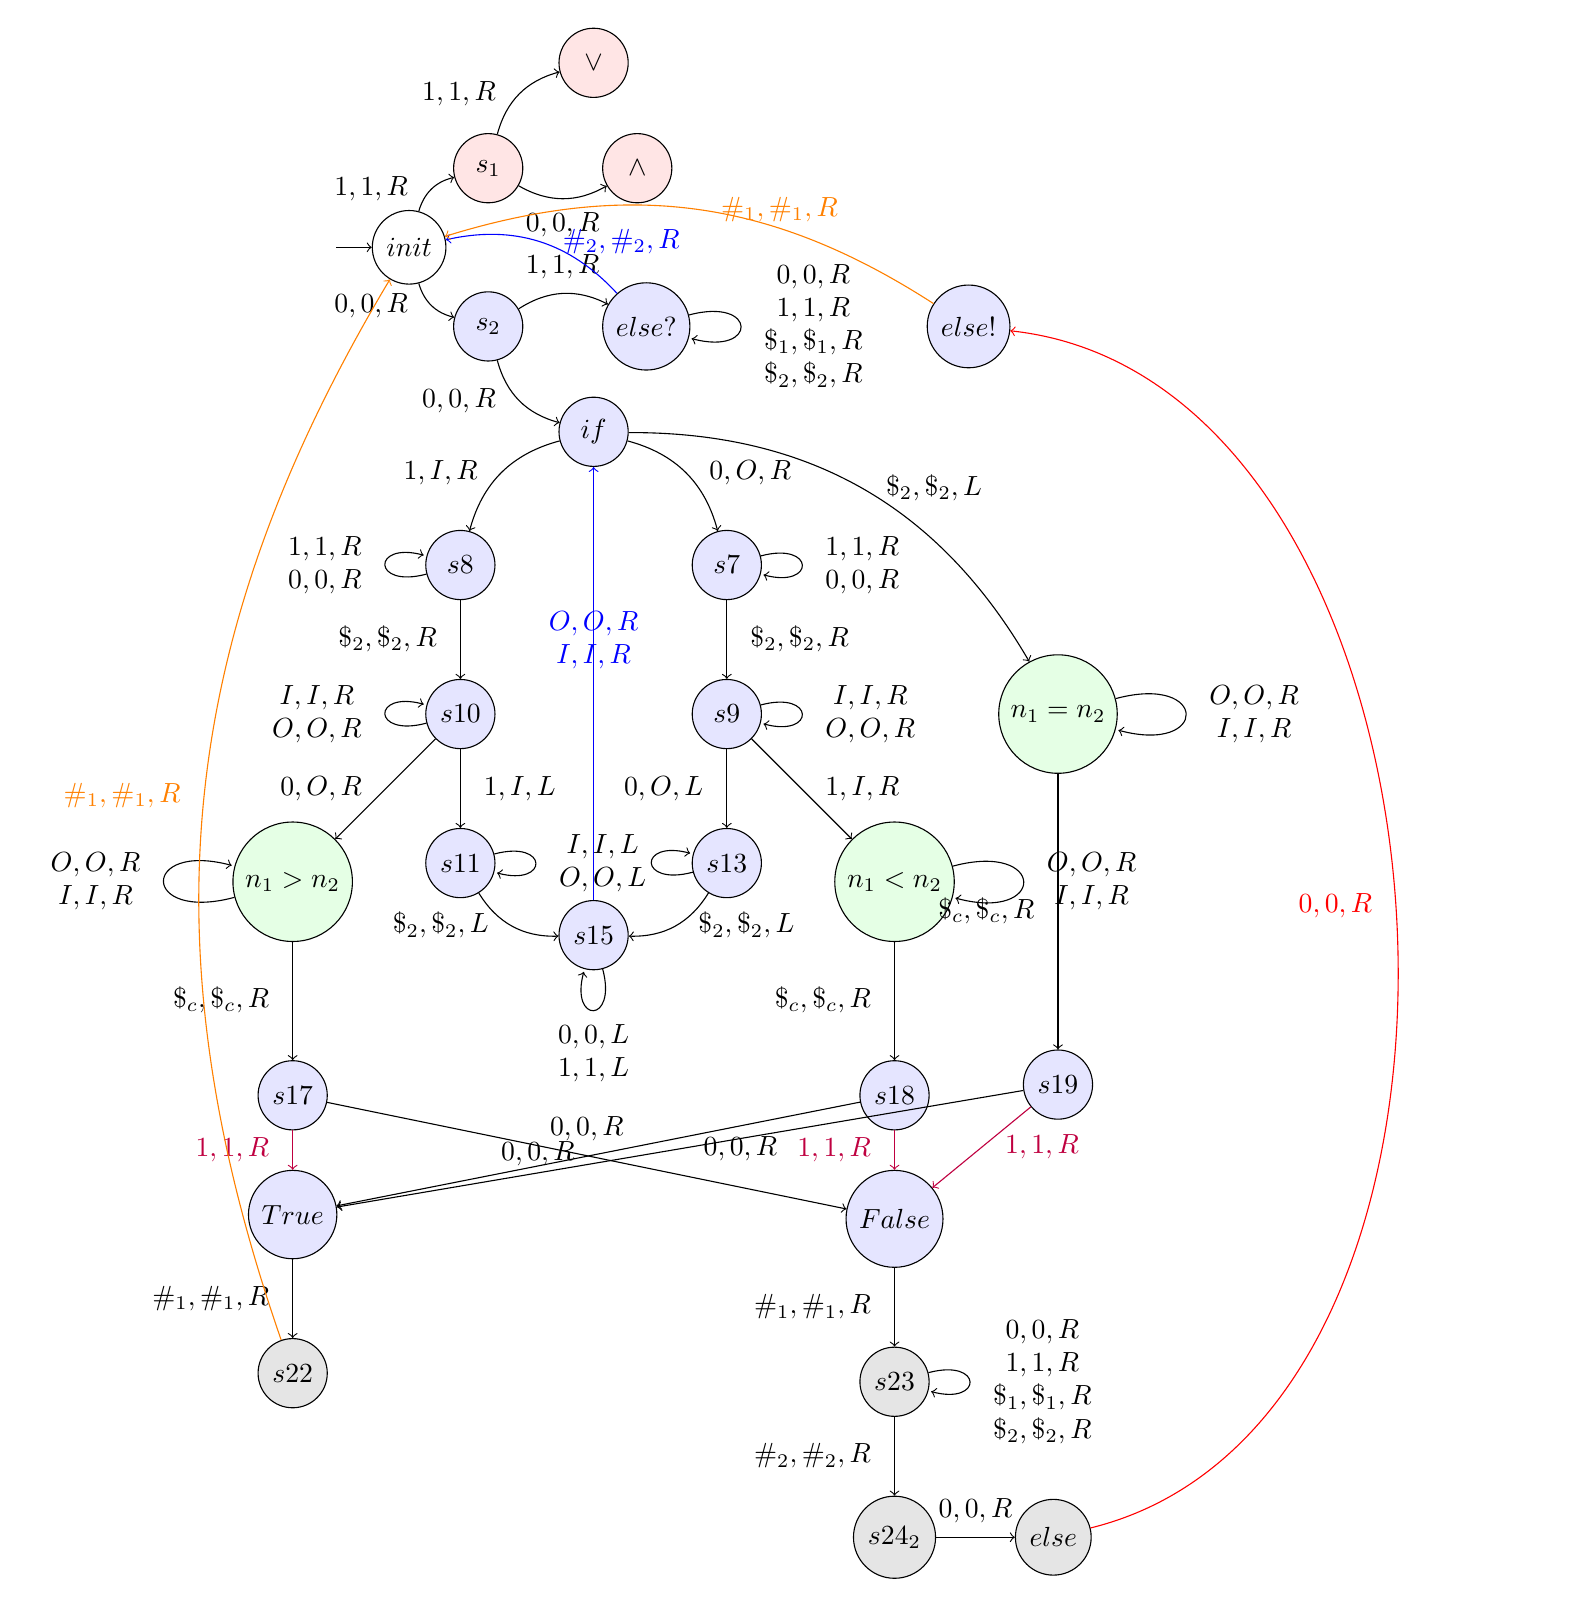
\begin{tikzpicture}
		
        \node[state, initial, initial text=] (s0) {$init$};
		\node[state] (s1) [above right=0.5of s0, fill=red!10] {$s_1$};
		\node[state] (s2) [below right=0.5of s0, fill=blue!10] {$s_2$};

        \node[state] (s3) [right=1of s2, fill=blue!10] {$else?$};
        \node[state] (s3_2) [right=3of s3, fill=blue!10] {$else!$};
		\node[state] (s4) [below right=1of s2, fill=blue!10] {$if$};

        \node[state] (s5) [right=1of s1, fill=red!10] {$\land$};
		\node[state] (s6) [above right=1of s1, fill=red!10] {$\lor$};

        \node[state] (s7) [below right=1.5 of s4, fill=blue!10] {$s7$};
        \node[state] (s8) [below left=1.5 of s4, fill=blue!10] {$s8$};
        \node[state] (s9) [below=1 of s7, fill=blue!10] {$s9$};
        \node[state] (s10) [below=1 of s8, fill=blue!10] {$s10$};
        \node[state] (s12) [below left=1.8 of s10, fill=green!10] {$n_1>n_2$};
        \node[state] (s11) [below=1 of s10, fill=blue!10] {$s11$};
        \node[state] (s13) [below =1 of s9, fill=blue!10] {$s13$};
        \node[state] (s14) [below right =1.8 of s9, fill=green!10] {$n_1<n_2$};
        \node[state] (s16) [right =3 of s9, fill=green!10] {$n_1=n_2$};
        \node[state] (s15) [below =5.5 of s4, fill=blue!10] {$s15$};

        \node[state] (s17) [below=1.5 of s12, fill=blue!10] {$s17$};
        \node[state] (s18) [below=1.5 of s14, fill=blue!10] {$s18$};
        \node[state] (s19) [below=3.5 of s16, fill=blue!10] {$s19$};
        \node[state] (s20) [below =0.5 of s17, fill=blue!10] {$True$};
        \node[state] (s21) [below =0.5 of s18, fill=blue!10] {$False$};

        \node[state] (s22) [below=1 of s20, fill=black!10] {$s22$};
        \node[state] (s23) [below=1 of s21, fill=black!10] {$s23$};
        \node[state] (s24) [below=1 of s23, fill=black!10] {$s24_2$};

        \node[state] (s24_2) [right=1 of s24, fill=black!10] {$else$};




		\path[->] 
        (s0) edge[left, bend left] node {$\begin{array}{c} 1,1,R\end{array}$} (s1)
        (s0) edge[left, bend right] node {$\begin{array}{c} 0,0,R\end{array}$} (s2)

        (s2) edge[above, bend left] node {$\begin{array}{c} 1,1,R\end{array}$} (s3)
        (s2) edge[left, bend right] node {$\begin{array}{c} 0,0,R\end{array}$} (s4)

        (s1) edge[below, bend right] node {$\begin{array}{c} 0,0,R\end{array}$} (s5)
        (s1) edge[left, bend left] node {$\begin{array}{c} 1,1,R\end{array}$} (s6)

        (s4) edge[right, bend left] node {$\begin{array}{c} 0,O,R\end{array}$} (s7)
        (s4) edge[left, bend right] node {$\begin{array}{c} 1,I,R\end{array}$} (s8)
        (s8) edge[left, loop left] node {$\begin{array}{c} 1,1,R \\ 0,0,R\end{array}$} (s8)
        (s7) edge[left, loop right] node {$\begin{array}{c} 1,1,R \\ 0,0,R\end{array}$} (s7)
        (s8) edge[left] node {$\begin{array}{c} \$_2,\$_2,R\end{array}$} (s10)
        (s7) edge[right] node {$\begin{array}{c} \$_2,\$_2,R\end{array}$} (s9)
        (s10) edge[left, loop left] node {$\begin{array}{c} I,I,R \\ O,O,R\end{array}$} (s8)
        (s9) edge[left, loop right] node {$\begin{array}{c} I,I,R \\ O,O,R\end{array}$} (s7)

        (s9) edge[right] node {$\begin{array}{c} 1,I,R\end{array}$} (s14)
        (s9) edge[left] node {$\begin{array}{c} 0,O,L\end{array}$} (s13)

        (s10) edge[right] node {$\begin{array}{c} 1,I,L\end{array}$} (s11)
        (s10) edge[left] node {$\begin{array}{c} 0,O,R\end{array}$} (s12)

        (s11) edge[left, loop right] node {$\begin{array}{c} I,I,L \\ O,O,L\end{array}$} (s11)
        (s13) edge[left, loop left] node {} (s13)
        (s11) edge[left, bend right] node {$\begin{array}{c} \$_2,\$_2,L\end{array}$} (s15)
        (s13) edge[right, bend left] node {$\begin{array}{c} \$_2,\$_2,L\end{array}$} (s15)
        (s15) edge[below, loop below] node {$\begin{array}{c} 0,0,L\\1,1,L\end{array}$} (s15)
        (s15) edge[draw=blue, above] node[blue] {$\begin{array}{c} O,O,R\\I,I,R\end{array}$} (s4)

        (s4)  edge[right, bend left] node {$\begin{array}{c} \$_2,\$_2,L\end{array}$} (s16)

        (s14) edge[loop right] node {$\begin{array}{c} O,O,R\\I,I,R\end{array}$} (s14)
        (s12) edge[loop left ] node {$\begin{array}{c} O,O,R\\I,I,R\end{array}$} (s12)
        (s16) edge[loop right] node {$\begin{array}{c} O,O,R\\I,I,R\end{array}$} (s16)

        (s12) edge[left] node {$\begin{array}{c} \$_c,\$_c,R \end{array}$} (s17)
        (s14) edge[left] node {$\begin{array}{c} \$_c,\$_c,R \end{array}$} (s18)
        (s16) edge[left] node {$\begin{array}{c} \$_c,\$_c,R \end{array}$} (s19)

        (s17) edge[left, draw=purple] node[purple] {$\begin{array}{c} 1,1,R \end{array}$} (s20)
        (s18) edge[left, draw=purple] node[purple] {$\begin{array}{c} 1,1,R \end{array}$} (s21)
        (s19) edge[right, draw=purple] node[purple] {$\begin{array}{c} 1,1,R \end{array}$} (s21)
        
        (s17) edge[above] node {$\begin{array}{c} 0,0,R \end{array}$} (s21)
        (s18) edge[left] node {$\begin{array}{c} 0,0,R \end{array}$} (s20)
        (s19) edge[right] node {$\begin{array}{c} 0,0,R \end{array}$} (s20)

        (s20) edge[left] node {$\begin{array}{c} \#_1,\#_1,R \end{array}$} (s22)
        (s21) edge[left] node {$\begin{array}{c} \#_1,\#_1,R \end{array}$} (s23)
        (s23) edge[loop right] node {$\begin{array}{c} 0,0,R\\1,1,R\\ \$_1,\$_1,R\\\$_2,\$_2,R \end{array}$} (s23)
        (s23) edge[left] node {$\begin{array}{c} \#_2,\#_2,R \end{array}$} (s24)
        (s24_2) edge[bend right=80, draw=red, left] node[red] {$\begin{array}{c} 0,0,R \end{array}$} (s3_2)
        (s24) edge[above] node {$\begin{array}{c} 0,0,R \end{array}$} (s24_2)
        (s3) edge[loop right] node {$\begin{array}{c} 0,0,R\\1,1,R\\ \$_1,\$_1,R\\\$_2,\$_2,R \end{array}$} (s3)
        (s3) edge[right, bend right, draw=blue] node[blue] {$\begin{array}{c} \#_2,\#_2,R \end{array}$} (s0)
        
        (s3_2) edge[right, bend right=25, draw=orange] node[orange] {$\begin{array}{c} \#_1,\#_1,R \end{array}$} (s0)
        (s22) edge[left, bend left=25, draw=orange] node[orange] {$\begin{array}{c} \#_1,\#_1,R \end{array}$} (s0);

        

    \end{tikzpicture}
    \end{center}
    }
$\\$
Dobbiamo considerare allora due aspetti:
\begin{itemize}
    \item Per effettuare l'AND logico elemento per elemento, sarà sufficiente andare a controllare che ad ogni passo $i$-esimo ci sia un termine a 1 e 1 per scrivere 1
    \item Per effettuare l'OR logico elemento per elemento, sarà sufficiente andare a controllare che ad ogni passo $i$-esimo ci sia almeno un termine a 1 per scrivere 1.
    \item Scriveremo il risultato nella seconda parola: se questa è la fine del programma, cancelleremo tutto quello che la precede.
\end{itemize}
Utilizziamo dapprima il codice per l'AND della precedente esercitazione. \textbf{Si assume che in input siano presenti parole di lunghezza uguale}:

\end{osservazioni}
\NewPageHeader
\begin{osservazioni}


        {
        \tikzset{state/.append style={minimum size=6mm, inner sep=1pt}}

        \begin{center}
    	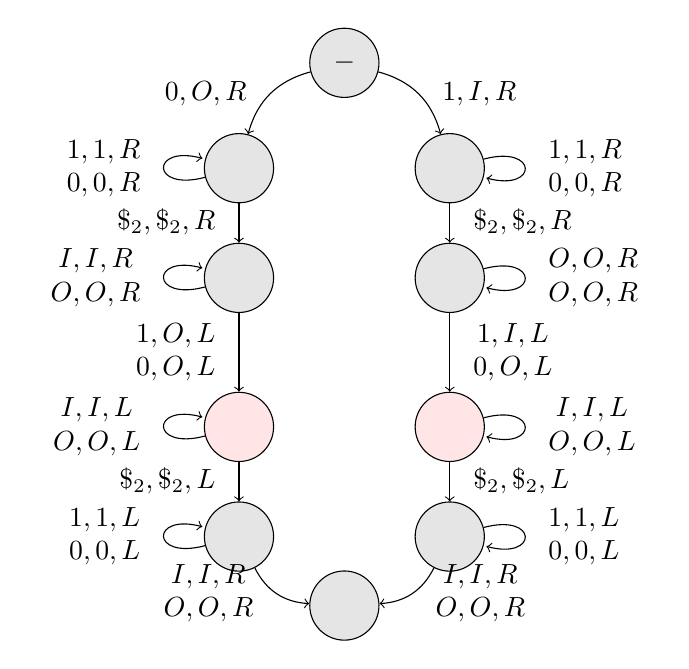
\begin{tikzpicture}
            
            \node[state] (A) [fill = black!10] {$-$}; %I
            \node[state] (B) [fill = black!10, below left=1of A] {};  %L
            \node[state] (C) [fill = black!10, below right=1of A] {}; %M
            
            \node[state] (D) [fill = black!10, below=0.5of B] {}; %N
            \node[state] (E) [fill = black!10, below=0.5of C] {}; % O
            
            \node[state] (F) [fill = red!10, below=1of D] {}; %P
            \node[state] (G) [fill = red!10, below=1of E] {}; %Q
            
            \node[state] (F1) [fill = black!10, below=0.5of F] {}; %R
            \node[state] (G1) [fill = black!10, below=0.5of G] {}; %S

            %\node[state] (T) [fill = black!10, below=1.5of R];
            %\node[state] (U) [fill = black!10, below=1.5of S];

            %\node[state] (T) [fill = black!10, below=1.5of R];
            %\node[state] (U) [fill = black!10, below=1.5of S];

            \node[state] (G2) [fill = black!10, below=6of A] {};
            
            \path[->]
            (A) edge [left, bend right] node {$\begin{array}{c} 0,O,R \end{array}$} (B)
            (A) edge [right, bend left] node {$\begin{array}{c} 1,I,R \end{array}$} (C)
            
            (B) edge [left, loop left] node {$\begin{array}{c} 1,1,R\\ 0,0,R \end{array}$} (B)
            (C) edge [right, loop right] node {$\begin{array}{c} 1,1,R\\ 0,0,R \end{array}$} (C)

            (B) edge [left] node {$\begin{array}{c} \$_2,\$_2,R \end{array}$} (D)
            (C) edge [right] node {$\begin{array}{c} \$_2,\$_2,R \end{array}$} (E)

            (D) edge [left] node {$\begin{array}{c} 1,O,L\\ 0,O,L  \end{array}$} (F)
            (E) edge [right] node {$\begin{array}{c} 1,I,L\\ 0,O,L \end{array}$} (G)

            (D) edge [loop left, left] node {$\begin{array}{c} I,I,R\\ O,O,R  \end{array}$} (D)
            (E) edge [loop right, right] node {$\begin{array}{c} O,O,R\\ O,O,R \end{array}$} (O)

            (F) edge [left] node {$\begin{array}{c} \$_2,\$_2,L  \end{array}$} (F1)
            (G) edge [right] node {$\begin{array}{c} \$_2,\$_2,L  \end{array}$} (G1)

            (F) edge [loop left, left] node {$\begin{array}{c} I,I,L\\ O,O,L  \end{array}$} (F)
            (G) edge [loop right, right] node {$\begin{array}{c} I,I,L\\ O,O,L \end{array}$} (G)

            (F1) edge [loop left, left] node {$\begin{array}{c} 1,1,L\\ 0,0,L  \end{array}$} (F1)
            (G1) edge [loop right, right] node {$\begin{array}{c} 1,1,L\\ 0,0,L \end{array}$} (G1)

            (F1) edge [bend right, left] node {$\begin{array}{c} I,I,R\\ O,O,R \end{array}$} (G2)
            (G1) edge [bend left, right] node {$\begin{array}{c} I,I,R\\ O,O,R \end{array}$} (G2);

        
        \end{tikzpicture}
        \end{center}
        }

Possiamo allora generalizzare anche il caso OR a partire da questo:


        {
        \tikzset{state/.append style={minimum size=6mm, inner sep=1pt}}

        \begin{center}
    	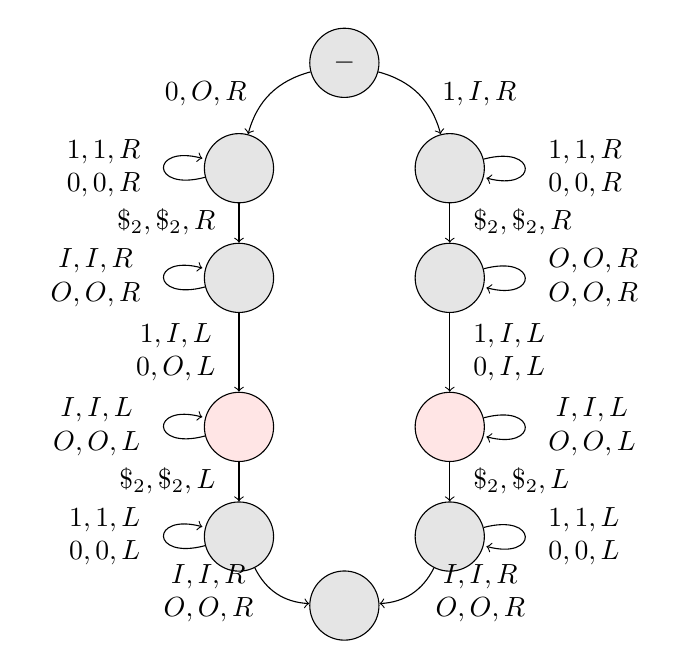
\begin{tikzpicture}
            
            \node[state] (I) [fill = black!10] {$-$};
            \node[state] (L) [fill = black!10, below left=1of I] {}; 
            \node[state] (M) [fill = black!10, below right=1of I] {};
            
            \node[state] (N) [fill = black!10, below=0.5of L] {};
            \node[state] (O) [fill = black!10, below=0.5of M] {};
            
            \node[state] (P) [fill = red!10, below=1of N] {};
            \node[state] (Q) [fill = red!10, below=1of O] {};
            
            \node[state] (R) [fill = black!10, below=0.5of P] {};
            \node[state] (S) [fill = black!10, below=0.5of Q] {};

            %\node[state] (T) [fill = black!10, below=1.5of R];
            %\node[state] (U) [fill = black!10, below=1.5of S];

            %\node[state] (T) [fill = black!10, below=1.5of R];
            %\node[state] (U) [fill = black!10, below=1.5of S];

            \node[state] (V) [fill = black!10, below=6of I] {};
            
            \path[->]
            (I) edge [left, bend right] node {$\begin{array}{c} 0,O,R \end{array}$} (L)
            (I) edge [right, bend left] node {$\begin{array}{c} 1,I,R \end{array}$} (M)
            
            (L) edge [left, loop left] node {$\begin{array}{c} 1,1,R\\ 0,0,R \end{array}$} (L)
            (M) edge [right, loop right] node {$\begin{array}{c} 1,1,R\\ 0,0,R \end{array}$} (M)

            (L) edge [left] node {$\begin{array}{c} \$_2,\$_2,R \end{array}$} (N)
            (M) edge [right] node {$\begin{array}{c} \$_2,\$_2,R \end{array}$} (O)

            (N) edge [left] node {$\begin{array}{c} 1,I,L\\ 0,O,L  \end{array}$} (P)
            (O) edge [right] node {$\begin{array}{c} 1,I,L\\ 0,I,L \end{array}$} (Q)

            (N) edge [loop left, left] node {$\begin{array}{c} I,I,R\\ O,O,R  \end{array}$} (N)
            (O) edge [loop right, right] node {$\begin{array}{c} O,O,R\\ O,O,R \end{array}$} (O)

            (P) edge [left] node {$\begin{array}{c} \$_2,\$_2,L  \end{array}$} (R)
            (Q) edge [right] node {$\begin{array}{c} \$_2,\$_2,L  \end{array}$} (S)

            (P) edge [loop left, left] node {$\begin{array}{c} I,I,L\\ O,O,L  \end{array}$} (P)
            (Q) edge [loop right, right] node {$\begin{array}{c} I,I,L\\ O,O,L \end{array}$} (Q)

            (R) edge [loop left, left] node {$\begin{array}{c} 1,1,L\\ 0,0,L  \end{array}$} (R)
            (S) edge [loop right, right] node {$\begin{array}{c} 1,1,L\\ 0,0,L \end{array}$} (S)

            (R) edge [bend right, left] node {$\begin{array}{c} I,I,R\\ O,O,R \end{array}$} (V)
            (S) edge [bend left, right] node {$\begin{array}{c} I,I,R\\ O,O,R \end{array}$} (V);

        
        \end{tikzpicture}
        \end{center}}


A questo punto, la MdT lascia il termine risolto al posto della seconda parola. Poiché ci interessa solamente dell'esecuzione dell'\textbf{ultimo} (per semplicità), possiamo verificare se la codifica del programma è terminata: controlliamo che dopo $\#_2$ ci sia $\sqcup$.
Per semplicità, li indicheremo con dei blocchi, che faranno riferimento a queste sottoporzioni.\\

Se così, vorremo tenere nel nastro solamente la parola: 
\begin{itemize}
    \item Cancelleremo qualsiasi cosa dal nastro, tranne quanto contenuto tra l'ultimo $\$_2...\#_2$
    \item Poi, sarà possibile riscrivere la parola all'inizio, ma lo eviteremo per semplicità.
\end{itemize}

\end{osservazioni}
\NewPageHeader
\begin{osservazioni}
\textbf{MdT Finale}:
\\
    {
    \tikzset{state/.append style={minimum size=6mm, inner sep=1pt}}

    \small
    \begin{center}
	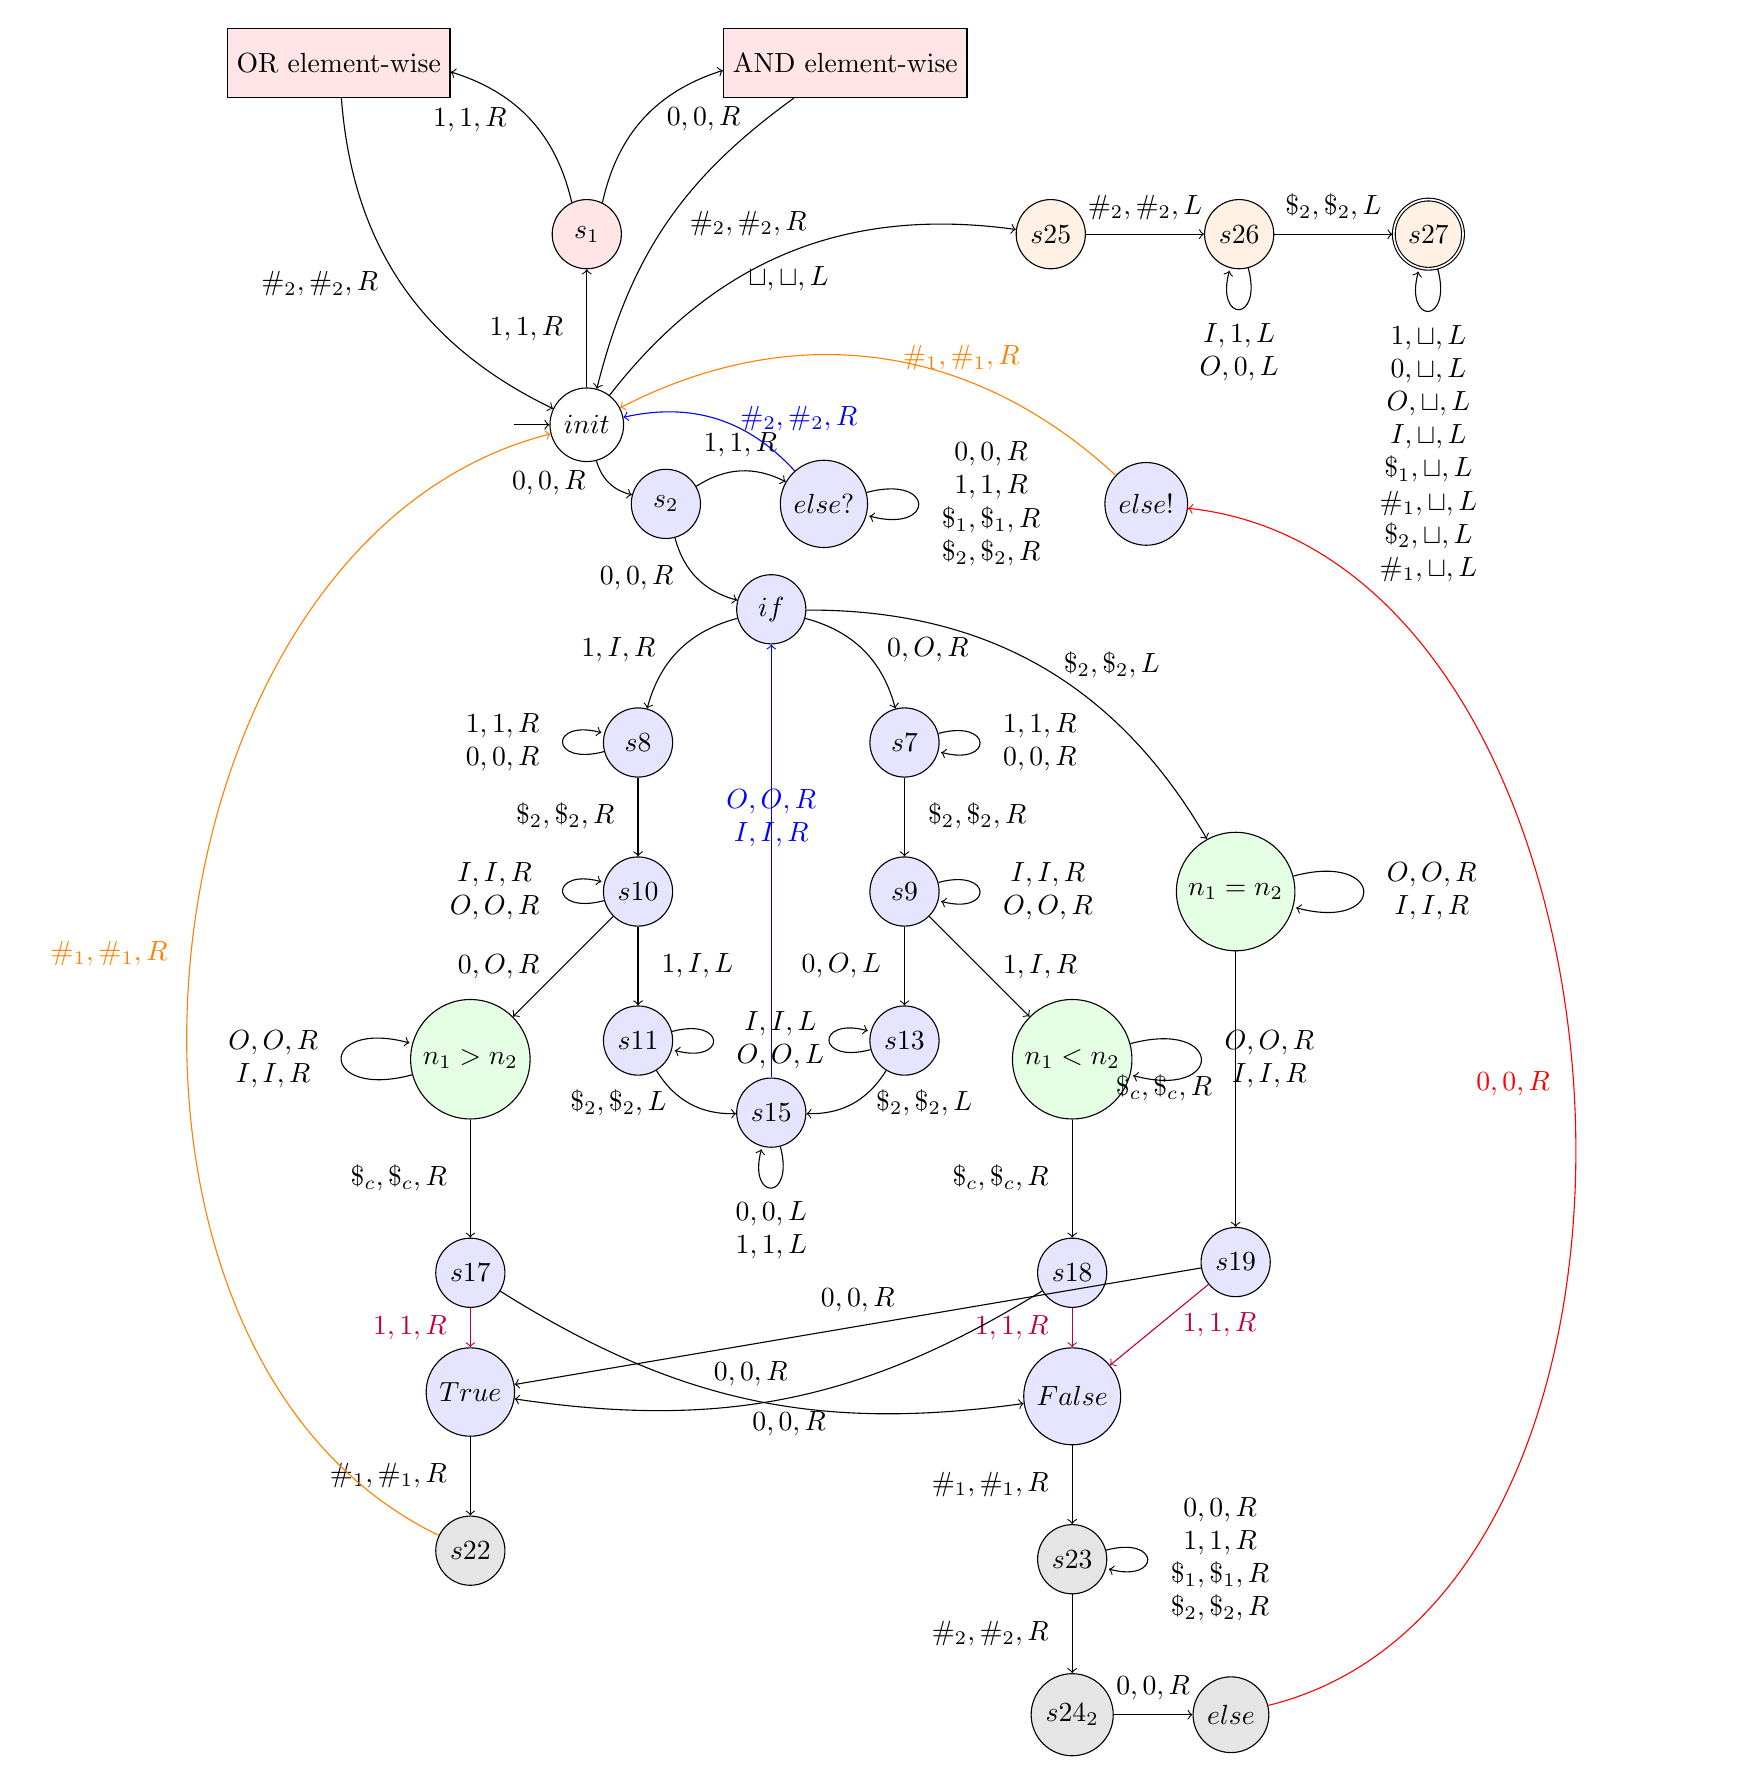
\begin{tikzpicture}
		
        \node[state, initial, initial text=] (s0) {$init$};
		\node[state] (s1) [above=1.5 and 0.5of s0, fill=red!10] {$s_1$};
		\node[state] (s2) [below right=0.5of s0, fill=blue!10] {$s_2$};

        \node[state] (s3) [right=1of s2, fill=blue!10] {$else?$};
        \node[state] (s3_2) [right=3of s3, fill=blue!10] {$else!$};
		\node[state] (s4) [below right=1of s2, fill=blue!10] {$if$};

        \node[state,rectangle] (s5) [above right= 2of s1, fill=red!10] {AND element-wise};
		\node[state, rectangle] (s6) [above left=2 of s1, fill=red!10] {OR element-wise};

        \node[state] (s7) [below right=1.5 of s4, fill=blue!10] {$s7$};
        \node[state] (s8) [below left=1.5 of s4, fill=blue!10] {$s8$};
        \node[state] (s9) [below=1 of s7, fill=blue!10] {$s9$};
        \node[state] (s10) [below=1 of s8, fill=blue!10] {$s10$};
        \node[state] (s12) [below left=1.8 of s10, fill=green!10] {$n_1>n_2$};
        \node[state] (s11) [below=1 of s10, fill=blue!10] {$s11$};
        \node[state] (s13) [below =1 of s9, fill=blue!10] {$s13$};
        \node[state] (s14) [below right =1.8 of s9, fill=green!10] {$n_1<n_2$};
        \node[state] (s16) [right =3 of s9, fill=green!10] {$n_1=n_2$};
        \node[state] (s15) [below =5.5 of s4, fill=blue!10] {$s15$};

        \node[state] (s17) [below=1.5 of s12, fill=blue!10] {$s17$};
        \node[state] (s18) [below=1.5 of s14, fill=blue!10] {$s18$};
        \node[state] (s19) [below=3.5 of s16, fill=blue!10] {$s19$};
        \node[state] (s20) [below =0.5 of s17, fill=blue!10] {$True$};
        \node[state] (s21) [below =0.5 of s18, fill=blue!10] {$False$};

        \node[state] (s22) [below=1 of s20, fill=black!10] {$s22$};
        \node[state] (s23) [below=1 of s21, fill=black!10] {$s23$};
        \node[state] (s24) [below=1 of s23, fill=black!10] {$s24_2$};

        \node[state] (s24_2) [right=1 of s24, fill=black!10] {$else$};

        \node[state] (s25) [right=5 of s1, fill=orange!10] {$s25$};
	    \node[state] (s26) [right=1.5 of s25, fill=orange!10] {$s26$};
        \node[state, accepting] (s27) [right=1.5 of s26, fill=orange!10] {$s27$};




		\path[->] 
        (s0) edge[left] node {$\begin{array}{c} 1,1,R\end{array}$} (s1)
        (s0) edge[left, bend right] node {$\begin{array}{c} 0,0,R\end{array}$} (s2)

        (s2) edge[above, bend left] node {$\begin{array}{c} 1,1,R\end{array}$} (s3)
        (s2) edge[left, bend right] node {$\begin{array}{c} 0,0,R\end{array}$} (s4)

        (s1) edge[right, bend left] node {$\begin{array}{c} 0,0,R\end{array}$} (s5)
        (s1) edge[left, bend right] node {$\begin{array}{c} 1,1,R\end{array}$} (s6)

        (s4) edge[right, bend left] node {$\begin{array}{c} 0,O,R\end{array}$} (s7)
        (s4) edge[left, bend right] node {$\begin{array}{c} 1,I,R\end{array}$} (s8)
        (s8) edge[left, loop left] node {$\begin{array}{c} 1,1,R \\ 0,0,R\end{array}$} (s8)
        (s7) edge[left, loop right] node {$\begin{array}{c} 1,1,R \\ 0,0,R\end{array}$} (s7)
        (s8) edge[left] node {$\begin{array}{c} \$_2,\$_2,R\end{array}$} (s10)
        (s7) edge[right] node {$\begin{array}{c} \$_2,\$_2,R\end{array}$} (s9)
        (s10) edge[left, loop left] node {$\begin{array}{c} I,I,R \\ O,O,R\end{array}$} (s8)
        (s9) edge[left, loop right] node {$\begin{array}{c} I,I,R \\ O,O,R\end{array}$} (s7)

        (s9) edge[right] node {$\begin{array}{c} 1,I,R\end{array}$} (s14)
        (s9) edge[left] node {$\begin{array}{c} 0,O,L\end{array}$} (s13)

        (s10) edge[right] node {$\begin{array}{c} 1,I,L\end{array}$} (s11)
        (s10) edge[left] node {$\begin{array}{c} 0,O,R\end{array}$} (s12)

        (s11) edge[left, loop right] node {$\begin{array}{c} I,I,L \\ O,O,L\end{array}$} (s11)
        (s13) edge[left, loop left] node {} (s13)
        (s11) edge[left, bend right] node {$\begin{array}{c} \$_2,\$_2,L\end{array}$} (s15)
        (s13) edge[right, bend left] node {$\begin{array}{c} \$_2,\$_2,L\end{array}$} (s15)
        (s15) edge[below, loop below] node {$\begin{array}{c} 0,0,L\\1,1,L\end{array}$} (s15)
        (s15) edge[draw=blue, above] node[blue] {$\begin{array}{c} O,O,R\\I,I,R\end{array}$} (s4)

        (s4)  edge[right, bend left] node {$\begin{array}{c} \$_2,\$_2,L\end{array}$} (s16)

        (s14) edge[loop right] node {$\begin{array}{c} O,O,R\\I,I,R\end{array}$} (s14)
        (s12) edge[loop left ] node {$\begin{array}{c} O,O,R\\I,I,R\end{array}$} (s12)
        (s16) edge[loop right] node {$\begin{array}{c} O,O,R\\I,I,R\end{array}$} (s16)

        (s12) edge[left] node {$\begin{array}{c} \$_c,\$_c,R \end{array}$} (s17)
        (s14) edge[left] node {$\begin{array}{c} \$_c,\$_c,R \end{array}$} (s18)
        (s16) edge[left] node {$\begin{array}{c} \$_c,\$_c,R \end{array}$} (s19)

        (s17) edge[left, draw=purple] node[purple] {$\begin{array}{c} 1,1,R \end{array}$} (s20)
        (s18) edge[left, draw=purple] node[purple] {$\begin{array}{c} 1,1,R \end{array}$} (s21)
        (s19) edge[right, draw=purple] node[purple] {$\begin{array}{c} 1,1,R \end{array}$} (s21)
        
        (s17) edge[above, bend right=20] node {$\begin{array}{c} 0,0,R \end{array}$} (s21)
        (s18) edge[below, bend left=20] node {$\begin{array}{c} 0,0,R \end{array}$} (s20)
        (s19) edge[above] node {$\begin{array}{c} 0,0,R \end{array}$} (s20)

        (s20) edge[left] node {$\begin{array}{c} \#_1,\#_1,R \end{array}$} (s22)
        (s21) edge[left] node {$\begin{array}{c} \#_1,\#_1,R \end{array}$} (s23)
        (s23) edge[loop right] node {$\begin{array}{c} 0,0,R\\1,1,R\\ \$_1,\$_1,R\\\$_2,\$_2,R \end{array}$} (s23)
        (s23) edge[left] node {$\begin{array}{c} \#_2,\#_2,R \end{array}$} (s24)
        (s24_2) edge[bend right=80, draw=red, left] node[red] {$\begin{array}{c} 0,0,R \end{array}$} (s3_2)
        (s24) edge[above] node {$\begin{array}{c} 0,0,R \end{array}$} (s24_2)
        (s3) edge[loop right] node {$\begin{array}{c} 0,0,R\\1,1,R\\ \$_1,\$_1,R\\\$_2,\$_2,R \end{array}$} (s3)
        (s3) edge[right, bend right, draw=blue] node[blue] {$\begin{array}{c} \#_2,\#_2,R \end{array}$} (s0)
        
        (s3_2) edge[right, bend right=35, draw=orange] node[orange] {$\begin{array}{c} \#_1,\#_1,R \end{array}$} (s0)
        (s22) edge[left, bend left=70, draw=orange] node[orange] {$\begin{array}{c} \#_1,\#_1,R \end{array}$} (s0)

        (s0) edge[below, bend left=30] node {$\begin{array}{c} \sqcup,\sqcup,L \end{array}$} (s25)
        (s25) edge[above] node {$\begin{array}{c} \#_2,\#_2,L \end{array}$} (s26)
        (s26) edge[above, loop below] node {$\begin{array}{c} I,1,L\\O,0,L \end{array}$} (s26)
        (s26) edge[above] node {$\begin{array}{c} \$_2,\$_2,L \end{array}$} (s27)
        (s27) edge[above, loop below] node {$\begin{array}{c} 1,\sqcup,L\\ 0,\sqcup,L \\ O,\sqcup,L \\I,\sqcup,L\\ \$_1,\sqcup,L \\ \#_1,\sqcup,L \\ \$_2,\sqcup,L \\ \#_1,\sqcup,L \\ 
        \end{array}$} (s27)

        (s6) edge[left, bend right] node {$\begin{array}{c} \#_2,\#_2,R \end{array}$} (s0)
        (s5) edge[bend right=20,right] node {$\begin{array}{c} \#_2,\#_2,R \end{array}$} (s0);

    \end{tikzpicture}
    \end{center}
    }
\end{osservazioni}






\vfill
\noindent\makebox[\linewidth]{\rule{\linewidth}{0.1pt}}



\end{document}